\section{Ideal Gases}

\subsection{gas molecules}


\subsubsection{motion of gas particles} \label{s-gas-intro}

\begin{wrapfigure}{r}{6.5cm}
	\centering
	
	\vspace*{-20pt}
	
	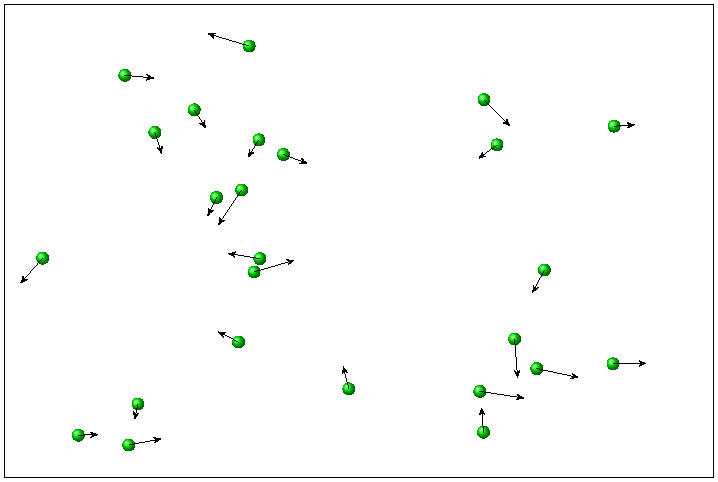
\includegraphics[width=6cm]{gas-random-motion}
		
	motion of gas molecules in a container
	
\end{wrapfigure}

gas consists of a large number of molecules

gas molecules move \emph{randomly} at high speeds

\cmt randomness results from \emph{collisions} of fast-moving molecules in the gas

for an individual molecule, its velocity changes constantly as it collides with other molecules

for the gas at any instant, there is a range of velocities for molecules

\cmt experimental evidence of random motion: \keypoint{Brownian motion}\index{Brownian motion}

dust or smoke particles in air undergo jerky random motion (viewed through microscope)

this is due to collisions with gas molecules that move randomly

\cmt speed of gas molecules depend on temperature

molecules move faster at higher temperature\footnote{We will prove this statement later in this chapter.}


\subsubsection{amount of molecules}

there are a huge number of molecules in a gas

we introduce \keypoint{amount of substance}\index{amount of substance} to measure the size of a collection of particles

\cmt unit of amount of substance: $[n] = \text{mol}$

\begin{ilight}
	one \keypoint{mole} is defined as the amount carbon-12 atoms in a sample of 12 grams
\end{ilight}

\cmt 1 mole of substance contains 6.02$\times$10$^{23}$ particles

this number is called \keypoint{Avogadro constant}\index{Avogadro constant}: $N_A = 6.02\times10^{23} \text{ mol}^{-1}$ \footnote{In 2018, IUPAC suggested a new definition of the mole, which is defined to contain exactly 6.02$\times$10$^{23}$ particles. This new definition fixed numerical value of the Avogadro constant, and emphasized that the quantity `amount of substance' is concerned with counting number of particles rather than measuring the mass of a sample.}

conversion between number of molecules and amount of substance: $\boxed{N=nN_A}$

\cmt it is useful to introduce the notion of molar mass $M$

\begin{ilight}
	\keypoint{molar mass}\index{molar mass} of a substance is defined as the mass of a given sample divided by the amount of substance: $M=\frac{m}{n}$
\end{ilight}

\begin{compactitem}
	\item[--] $\text{amount of substance} = \frac{\text{mass of sample}}{\text{molar mass}}$, or $n = \frac{m}{M}$
	
	\eqyskip
	
	\item[--] $\text{mass of single molecule} = \frac{\text{molar mass}}{\text{Avogadro constant}}$, or $m_0 = \frac{M}{N_A}$
\end{compactitem}

\example{Find the number of molecules in 160 grams of argon-40 gas.}

\sol amount of gas: $n=\frac{m}{M} = \frac{160 \text{ g}}{40 \text{ g mol}^{-1}} = 4.0 \text{ mol}$

number of gas molecules: $N = n N_A = 4.0 \text{ mol} \times 6.02\times10^{23} \text{ mol}^{-1} \approx 2.41 \times 10^{24}$ \eoe

\question{Find the mass of a sample of uranium-235 that contains $6.0\times10^{20}$ atoms.}
	




\subsubsection{pressure (qualitative view)}

when gas molecules collide with walls of container and rebound, they are acted by a force

by Newton's third law, gas molecules must exert a reaction force on container in return

contributions from many molecules give rise to a pressure

\example{If a gas is heated with its volume fixed, how does the pressure change?}

\sol at higher temperature, gas molecules move faster

they will collide \emph{harder} and produce a greater force upon each collision

they will also collide more \emph{frequently} with the container

so pressure of the gas will increase \eoe

\question{If you pump gas into a bicycle tyre, state and explain how the pressure changes.}

\question{A fixed amount of gas is allowed to expand at constant temperature, state and explain how the pressure changes.}



\subsection{ideal gas}

\subsubsection{ideal gas equation}

\rcyskip

\begin{ilight}
	a gas that satisfies the equation $\boxed{pV=nRT}$ or $\boxed{pV=NkT}$ at any pressure $p$, any volume $V$, and thermodynamic temperature $T$ is called an \keypoint{ideal gas}\index{ideal gas}
\end{ilight}

\keypoint{molar gas constant}: $R=8.31 \text{ J mol}^{-1}\text{ K}^{-1}$

\keypoint{Boltzmann constant}: $k=1.38\times10^{-23} \text{ J K}^{-1}$

values of $R$ and $k$ apply for any ideal gas, i.e., they are \emph{universal} constants

\cmt recall conversion between number of molecules and amount of substance: $\boxed{N=nN_A}$

we have relation between the constants: $R = kN_A$, or $k=\frac{R}{N_A}$

\cmt one must use \emph{thermodynamic temperature} in the equation

thermodynamic temperature is measured in kelvins (K), so it is also called the \emph{Kelvin scale}\footnote{We will discuss in details about Kelvin scale in \S\ref{s-temp-scale} and \S\ref{s-abs-zero}.}

conversion between Kelvin temperature and Celsius temperature: $\boxed{T_K (\text{K}) \text{ } \autorightleftharpoons{\footnotesize -273}{\footnotesize +273} \text{ } T_C (\OC)}$

\subsubsection*{real gases}

real gas behaves ideally at sufficiently high temperature and low pressure

\begin{compactitem}
	\item[--] at very low temperatures, real gas will condense into liquid or solid
	
	\item[--] at very high pressures, intermolecular forces become important
\end{compactitem}

however, under normal conditions (room temperature $T \approx 300 \text{ K}$ and standard atmospheric pressure $p \approx 1.0\times10^5 \text{ Pa}$), there is no significant difference between a real gas and an ideal gas

so ideal gas approximation can be used with good accuracy for most of our applications

\example{A sealed cylinder of volume of 0.050 m$^3$ contains 75 g of air. The molar mass of air is 29 g mol$^{-1}$. (a) Find the air pressure when its temperature is $30^\circ$C. (b) The gas is allowed to expand with its pressure fixed. Find the temperature of the gas when the volume doubles.}

\sol amount of gas: $n=\frac{m}{M} = \frac{75}{29} \approx 2.59 \text{ mol}$

\eqyskip

pressure at $30^\circ$C: $p = \frac{nRT_1}{V_1} = \frac{2.59\times8.31\times(30+273)}{0.050} \approx 1.30\times10^5 \text{ Pa}$

\eqyskip

pressure fixed, so $V \propto T \RA \frac{T_2}{T_1} = \frac{V_2}{V_1} = 2 \RA T_2 = 2\times (30+273) = 606 \text{ K} = 333^\circ\text{C}$ \eoe

\example{A gas cylinder holding 5000 cm$^3$ of air at a temperature of 27 $^\circ$C and a pressure of $6.0\times10^5 \text{ Pa}$ is used to fill balloons. Each balloon contains 1000 cm$^3$ of air at 27 $^\circ$C and $1.0\times10^5$ Pa when filled. (a) Find the initial amount of gas in the cylinder. (b) Find the number of balloons that can be filled.}

\sol initial amount of gas in cylinder: $n_0 = \frac{p_0 V}{RT} = \frac{9.0\times10^5\times5000\times10^{-6}}{8.31\times(27+273)} \approx 1.203 \text{ mol}$

\eqyskip

final amount of gas in cylinder: $n_\text{remain} = \frac{pV}{RT} = \frac{1.0\times10^5\times5000\times10^{-6}}{8.31\times(27+273)} \approx 0.201 \text{ mol}$\footnote{Air will leave the cylinder to fill balloons only if pressure inside the cylinder is higher than pressure of the balloon. When the two pressures become equal, no more balloons can be filled, there will be some air remain in cylinder.}

\eqyskip

amount of gas in each balloon: $n_\text{b} = \frac{pV_b}{RT} = \frac{1.0\times10^5\times1000\times10^{-6}}{8.31\times(27+273)} \approx 0.040 \text{ mol}$

\eqyskip

number of balloons: $N = \frac{n_0 - n_\text{remain}}{n_\text{b}} = \frac{1.203-0.201}{0.040} \approx 25$ \eoe

\example{A storage cylinder has a volume of $5.0\times10^{-4}\text{ m}^3$. The gas is at a temperature
	of 300 K and a pressure of $4.0 \times 10^6$ Pa.	(a) Find the number of molecules in the cylinder. (b) The gas molecules slowly leak from the cylinder at a rate of $1.6 \times 10^{16} \text{ s}^{-1}$. Find the time, in days, after which the pressure will reduce by 5.0\%.}

\sol initial number of molecules: $N_0 = \frac{p_0V}{kT} = \frac{4.0\times10^6\times 5.0\times10^{-4}}{1.38\times10^{-23}\times300}\approx 4.83\times10^{23}$

\eqyskip

volume fixed, so $N \propto p \RA \frac{\Delta N}{N_0} = \frac{\Delta p}{p_0} = 5.0\%$

number of molecules escaped: $\Delta N = 0.05\times4.83\times10^{23} \approx 2.42 \times10^{22}$

time needed: $t = \frac{2.42 \times10^{22}}{1.6 \times 10^{16}} \approx 1.51 \times 10^6 \text{ s} \approx 17.4 \text{ days}$ \eoe

\newpage %%%%

\question{Containers $A$ has a volume of $2.5\times10^{-2} \text{ m}^3$ contains a gas at a temperature of 17$^\circ$C and pressure of $1.3 \times 10^5 \text{ Pa}$ and . Another container $B$ of same size holds a gas at same temperature and a pressure of $1.9 \times 10^5 \text{ Pa}$. The two containers are initially isolated from each another. (a) Find the total amount of molecules. (b) The two containers are now connected through a tube of negligible volume. Assume the temperature stays unchanged, find the final pressure of the gas.}

\question{The air in a car tyre can be assumed to have a constant volume of $3.0\times10^{-2} \text{ m}^3$}. The pressure of this air is $2.8\times10^5 \text{ Pa}$ at a temperature of $25^\circ$C. The pressure is to be increased using a pump. On each stroke 0.015 mol of air is forced into the tyre. If gas has a final pressure of $3.6\times10^5 \text{ Pa}$ and final temperature of $28^\circ$C. Find the number of strokes of the pump required.


\subsubsection{empirical laws}

historically, the ideal gas law was first stated by \emph{\'Emile Clapeyron} in 1834:

for a fixed amount of gas, $\boxed{\frac{PV}{T} = \text{const}}$

his work was based on the empirical Boyle's law, Charles's law, and Gay-Lussac's law

we will next recover these laws from the ideal gas equation

\subsubsection*{Boyle's law}\index{Boyle's law}

Boyle's law was discovered by \emph{Robert Boyle} in 1662, based on experimental observations

\begin{wrapfigure}{r}{5cm}
	\centering
	\vspace*{-10pt}
		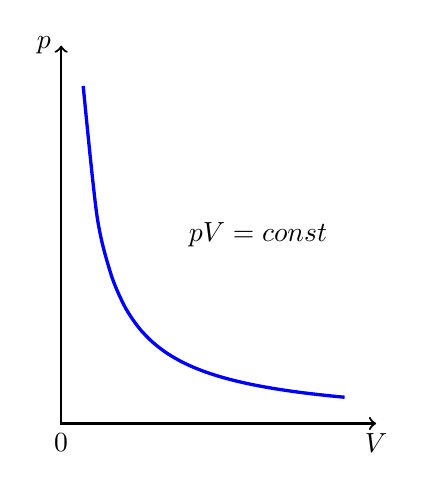
\begin{tikzpicture}[yscale=1.2]
		\draw [thick, <->] (0,4) node[left]{$p$} -- (0,0) node[below]{$0$} -- (4,0) node[below]{$V$};
		\draw [very thick,blue,domain=0.28:3.6,samples=20,smooth,variable=\x] plot (\x,{1/\x)});
		\draw (2.5,2) node{$pV=\text{const}$};
		\end{tikzpicture}
		\vspace*{-10pt}
\end{wrapfigure}

if temperature $T$ remains constant, then

{

\centering

$\boxed{pV=\text{const}}$, or $\boxed{p \propto \frac{1}{V}}$

} 

pressure $p$ of gas is inversely proportional to volume $V$

\cmt for a gas with fixed temperature: $p_1 V_1 = p_2 V_2$

\cmt a thermodynamic process for which temperature is kept constant is called an \emph{isothermal} process

$p$-$V$ relation for an isothermal process is shown




\subsubsection*{Charles's law}\index{Charles's law}

Charles's law was discovered by \emph{Jacques Charles} in 1787, based on experimental observations

\begin{figure}[ht]
	\centering
	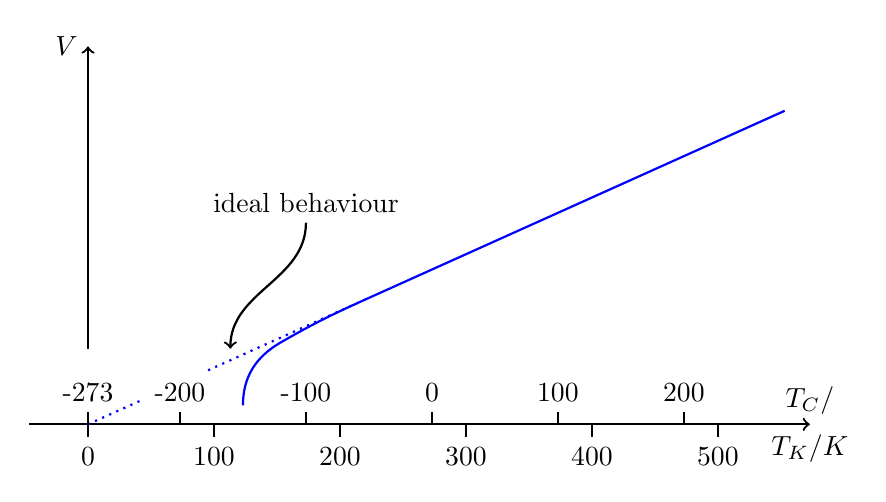
\begin{tikzpicture}[scale=1.6]
		\draw [thick, ->] (-2.73,0.6) -- (-2.73,3) node[left]{$V$};
		\draw [thick, ->] (-3.2,0) -- (3,0) node[below]{$T_K/\text{K}$} node[above]{$T_C/\OC$};
		\draw [thick,blue,domain=-0.5:2.8,samples=2,smooth,variable=\x] plot (\x,{0.45*(\x+2.73)});
		\draw [thick,blue,dotted,domain=-2.73:-0.5,samples=2,smooth,variable=\x] plot (\x,{0.45*(\x+2.73)});
		\draw [thick,blue] (-0.5,1.0035) to [out=204.2,in=30] (-1.2,0.65) to [out=210,in=90] (-1.5,0.15);
		\draw[white,fill] (-2.3,0.2) rectangle (-1.8,0.5);
		\foreach \s in {-200,-100,...,200}
		\draw [thick] (\s/100,0) --(\s/100,0.1) node[above]{\s};
		\foreach \s in {0,100,...,500}
		\draw [thick] (\s/100-2.73,0) -- (\s/100-2.73,-0.1) node[below]{\s};
		\draw [thick] (-2.73,0) -- (-2.73,0.1) node[above]{-273};
		\draw [<-, thick] (-1.6,0.6) to [out=90, in=270] (-1,1.6) node[above]{ideal behaviour};
	\end{tikzpicture}
\end{figure}

if pressure $p$ remains constant, then: $\boxed{\frac{V}{T}=\text{const}}$, or $\boxed{V \propto T}$

i.e., volume $V$ of gas is directly proportional to its temperature $T$

\cmt proportionality relation only applies if Kelvin scale is used

\cmt a thermodynamic process for which pressure is kept constant is called an \emph{isobaric} process

$V$-$T$ relation for an isobaric process is shown

\cmt Charles's law implies that volume of gas tends to zero at a certain temperature

historically this is how the idea of \emph{absolute zero} first arose

\cmt as $T\to0$, a real gas condenses into solid

there will be deviation from ideal behaviour (dotted line)



\subsubsection*{Gay-Lussac's law}\index{Gay-Lussac's law}

\begin{wrapfigure}{r}{4.5cm}
	\centering
	\vspace*{-40pt}
	\begin{tikzpicture}[scale=1]
	\draw [thick, <->] (0,4) node[left]{$p$} -- (0,0) node[below]{$0$} -- (4,0) node[below]{$T$};
	\draw [thick,blue] (1,1) -- (3.6,3.6);
	\draw [thick,dotted] (0,0) -- (1,1);
	\end{tikzpicture}
	\vspace*{-30pt}
\end{wrapfigure}

Gay-Lussac's law was discovered by \emph{Joseph Louis Gay-Lussac} between 1800 and 1802


if volume $V$ remains constant, then

{
	
	\centering
	
	$\boxed{\frac{p}{T}=\text{const}}$, or $\boxed{p \propto T}$
	
} 

i.e., pressure $p$ is directly proportional to temperature $T$

\cmt a thermodynamic process for which volume is kept constant is called an \emph{isochoric} process, or \emph{isometric} process

$p$-$T$ relation for an isochoric process is shown

\cmt behaviour of real gas again deviates from ideal behaviour (dotted line) as $T\to0$





\subsection{kinetic theory of ideal gases}

\keypoint{kinetic model of gases}\index{kinetic model of gases}: a theory based on microscopic motion of molecules of a gas that explains its macroscopic properties

\subsubsection{assumptions of ideal gas model}

\rcyskip

\begin{ilight}
	
kinetic theory of the ideal gas model is based on the following assumptions:

\begin{compactitem}
	
\item[--] gas molecules are in constant \emph{random} motion
	
\item[--] \emph{intermolecular separation} is much greater than size of molecules

volume of molecules is negligible compared to volume occupied by gas

\item[--] \emph{intermolecular forces} are negligible

\item[--] collisions between molecules are perfectly \emph{elastic}, i.e., no kinetic energy lost

\item[--] molecules travel in straight line between collisions
\end{compactitem}

\end{ilight}

\example{A mass of 20 g helium-4 at a temperature of 37$^\circ$C has a pressure of $1.2\times10^5 \text{ Pa}$. Each helium-4 atom has a diameter of 280 pm. (a) Find the volume occupied by the gas and the volume of atoms in this gas. (b) Compare the two volumes, suggest whether this gas can be considered as an ideal gas.}

\sol number of helium molecules: $N = nN_A = \frac{m}{M} \times N_A = \frac{20}{4.0} \times 6.02\times10^{23} \approx 3.01\times10^{24} $

\eqyskip

volume of gas: $V_\text{gas} = \frac{NkT}{p} = \frac{3.01\times10^{24}\times1.38\times10^{-23}\times (37+273)}{1.2\times10^5} \approx 0.107 \text{ m}^3$

\eqyskip

volume of one atom: $V_\text{atom} = \frac{4}{3}\pi r^3 = \frac{4}{3} \pi\times(140\times10^{-12})^3 \approx 1.15\times10^{-29} \text{ m}^3$

volume of all atoms: $V_\text{atoms} = N V_\text{atom} = 3.01\times10^{24} \times 1.15\times10^{-29} \text{ m}^3 \approx 3.46 \times 10^{-5} \text{ m}^{3}$

$V_\text{gas} \gg V_\text{atoms}$, so this gas can approximate to an ideal gas \eoe


\subsubsection{pressure (quantitative view)}

we are ready to derive a formula for pressure due to ideal gas

pressure of gas is due to collision of gas molecules with container

let's first consider the effect of one single molecule moving in one dimension only, and then generalise the result to a gas containing $N$ molecules moving in all three dimensions



\begin{figure}[ht]
\centering
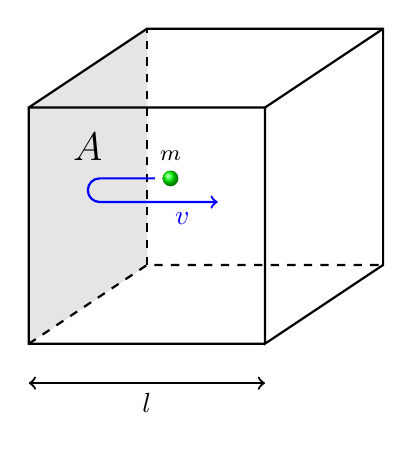
\begin{tikzpicture}[scale=1]
\coordinate (A) at (0,0); 
\coordinate (B) at (3,0);
\coordinate (C) at (4.5,1); 
\coordinate (D) at (1.5,1);
\coordinate (E) at (0,3); 
\coordinate (F) at (3,3);
\coordinate (G) at (4.5,4); 
\coordinate (H) at (1.5,4);
\draw [gray!20,fill] (A) -- (D) -- (H) -- (E) -- cycle;
\draw [thick] (B) -- (A) -- (E) -- (F) -- (B) -- (C) -- (G) -- (H) -- (E);
\draw [thick] (F) -- (G);
\draw [thick,dashed] (A) -- (D) -- (C);
\draw [thick,dashed] (D) -- (H);
\draw [thick,blue,->] (1.6,2.1) -- (0.9,2.1) to [out=180,in=90] (0.75,1.95)to [out=-90,in=180] (0.9,1.8) -- (2.4,1.8) node[below, pos=0.7]{$v$};
\shade [ball color = green] (1.8,2.1) circle [radius=0.1];
\draw [thick,<->] (0,-0.5) -- (1.5,-0.5) node[below]{$l$} -- (3,-0.5);
\node at (0.75,2.5) {{\Large $A$}};
\node[above] at (1.8,2.2) {{\footnotesize $m$}};
\end{tikzpicture}

one gas molecule moving in 1-D
\end{figure}

let's assume this single molecule only moves in $x$-direction (see figure)

change in momentum when colliding with wall: $\Delta P_x = mv_x - (-mv_x) = 2mv_x$\footnote{In this section we use $P$ for momentum of a particle and $p$ for pressure of a gas to avoid confusion.}

time interval between collisions: $\Delta t=\frac{2l}{v_x}$

average force acting: $F_x=\frac{\Delta P_x}{\Delta t} = \frac{2mv_x}{\tfrac{2l}{v_x}} = \frac{mv_x^2}{l}$

average pressure: $p_x=\frac{F}{A} = \frac{mv_x^2}{lA} = \RA p_x = \frac{mv_x^2}{V}$

generalisation to $N$ molecules moving in 3-D

\begin{compactitem}
	\item[--] $N$ molecules so $N$ times the contributions to pressure
	
	but there is a \emph{distribution} of speeds for $N$ molecules, so should take average of $v^2$
	
	\item[--] in three-dimensional space, we have: $v^2=v_x^2 + v_y^2 + v_z^2$
	
	but molecules have no preference in any specific direction, so: $\avg{v_x^2} = \avg{v_y^2} = \avg{v_z^2} = \frac{\avg{v^2}}{3}$
	
	pressure should be shared equally among three dimensions: $p=p_x=p_y=p_z$
		
\end{compactitem}


therefore we find the pressure of an ideal gas is given by: $\boxed{p = \frac{Nm\avg{v^2}}{3V}}$

\cmt $\avg{v^2}$ is the \emph{mean square velocity} of gas molecules

we can further define r.m.s. (root mean square) velocity: $v_\text{rms} = \sqrt{\avg{v^2}}$ 

gas molecules in random motion so there exists a range of velocities

we cannot tell exact velocity of a specific molecule, but can only tell mean values

\cmt $N$ is number of molecules, $m$ is mass of one molecule

then $Nm$ gives total mass of the gas, and $\frac{Nm}{V}$ gives gas density $\rho$

we can rewrite the pressure formula as: $\boxed{p=\frac{1}{3}\rho \avg{v^2}}$ 

(pressure depends only on density and mean square speed of molecules)

\cmt physical interpretation of the formula

\begin{compactitem}
\item[--] $N \up$ $\ra$ more molecules, more collisions $\ra p\up$

\item[--] $m \up$ $\ra$ greater mass, greater force upon collision $\ra p\up$

\item[--] $v \up$ $\ra$ strike container harder, also more often $\ra p\up$

\item[--] $V \up$ $\ra$ spend more time in gas, less frequent collision with container $\ra p\down$
\end{compactitem}


\subsubsection{kinetic energy}

we now have two equations for ideal gases:
\begin{equation*}
\left\{
	\begin{array}{ll}
	pV = nRT \, \text{, or } \, pV = NkT &\quad \text{ideal gas law} \\
	p = \frac{Nm\avg{v^2}}{3V} &\quad \text{pressure law}
	\end{array} \right.
\end{equation*}

compare the two equations: $pV=\frac{1}{3}Nm\avg{v^2}=NkT \RA m\avg{v^2}=3kT$

\emph{mean kinetic energy} of a single molecule in a gas is: $\boxed{\avg{E_k}=\frac{1}{2}m\avg{v^2}=\frac{3}{2}kT}$

mean K.E. of ideal gas molecules is \emph{proportional} to its thermodynamic temperature

\cmt useful relation for molecular speeds: $\boxed{v_\text{rms}^2 \propto T}$

recall our statement in \S\ref{s-gas-intro}, higher temperature means higher speed for molecules

\cmt we only talk about \emph{translational} K.E. here

molecules have this energy because they are moving through space

total kinetic energy may also include \emph{rotational} K.E. and \emph{vibrational} K.E.
\footnote{There is an important result in classical thermal physics, known as the \emph{equipartition of energy theorem}. It states that the average energy per molecule is $\frac{1}{2}kT$ for each independent \emph{degree of freedom}. A molecule can move in three directions, corresponding to three translational degrees of freedom, thus its mean translational kinetic energy is $\frac{3}{2}kT$. For a polyatomic gas (each molecule consists of several atoms), apart from translational motion , it has additional rotational degrees of freedom and different vibrational modes, so its average energy can be calculated by counting the total number of degrees of freedom.}

\cmt $\avg{E_k} = \frac{3}{2}k T$ gives the \emph{mean}, or \emph{average} K.E. per molecule

gas molecules exchange energies with each other upon collisions

for an individual molecule, its K.E. is not a constant

but mean K.E. is constant, which depends on temperature $T$ only

\cmt in a mixture of several gases, K.E. is shared \emph{equally} among its components

this is because of repeated collisions between particles

though all molecules have same K.E., heavier molecules will move more slowly




\example{Air consists of oxygen (O$_2$, molar mass $32\text{ g mol}^{-1}$) and nitrogen (N$_2$, molar mass $28\text{ g mol}^{-1}$). (a) Calculate the mean translational kinetic energy of these molecules at 300 K. (b) Estimate the typical speed for each type of the molecule.}

\sol mean K.E. of single molecule: $\avg{E_k} = \frac{3}{2}kT = \frac{3}{2} \times 1.38\times10^{-23} \times 300 \approx 6.21\times 10^{-21} \text{ J}$

{
	
	\centering
	
	$\avg{E_k} = \frac{1}{2}m\avg{v^2} = \frac{3}{2} kT \RA \frac{1}{2} \frac{M}{N_A} \avg{v^2} = \frac{3}{2} kT \RA \avg{v^2} = \frac{3kN_AT}{M} = \frac{3RT}{M}$
	
}

\eqyskip

for oxygen molecule: $v_\text{O$_2$} \approx  \sqrt{\frac{3\times8.31\times300}{0.032}} \approx 483 \mps$

\eqyskip

for nitrogen molecule: $v_\text{N$_2$} \approx  \sqrt{\frac{3\times8.31\times300}{0.028}} \approx 517 \mps$ \eoe

\example{A cylinder container initially holds a gas of helium-4 at a temperature of 54\OC. (a) Find the mean square speed of these helium atoms. (b) If the temperature is raised to 540\OC, find the r.m.s. speed of the atoms.}

\sol mass of one helium-4 atom: $m=4\text{u} = 4\times 1.66\times10^{-27} \approx 6.64\times10^{-27} \text{ kg}$

at 54\OC: $\, \frac{1}{2}m\avg{v^2} = \frac{3}{2}kT \RA \avg{v^2} = \frac{3kT}{m} = \frac{3\times1.38\times10^{-23}\times(54+273)}{6.64\times10^{-27}} \approx 2.04 \times 10^6 \text{ m}^2 \text{ s}^{-2}$

\eqyskip 

note relation between $v$ and $T$: $\, \avg{v^2} \propto T \RA \frac{\avg{v^{\prime 2}}}{\avg{v^2}} = \frac{T'}{T} \RA v'_\text{rms} = \sqrt{\frac{T'}{T}}\times v_\text{rms}$

\eqyskip 

at 540\OC: $\, v'_\text{rms} = \sqrt{\frac{540+273}{54+273}} \times \sqrt{2.04 \times 10^6} \approx 2.25 \times 10^3 \mps$ \eoe


\question{A fixed mass of gas expands to twice its volume at constant temperature. (a) How does its pressure change? (b) How does mean kinetic energy change?}

\question{In order for a molecule to escape from the gravitational field of the earth, it must have a speed of $1.1\times10^6\mps$ at the top of the atmosphere. (a) Estimate the temperature at which helium-4 atoms could have this speed. (b) Helium atom actually escape from top of the atmosphere at much lower temperatures, explain how this is possible.}